% ============================================================================
% CHAPTER 1D: ELECTROMECHANICAL SYSTEMS
% ============================================================================

\section{Electromechanical Systems}
\label{sec:electromechanical}

Electromechanical systems convert between electrical and mechanical energy. They are ubiquitous in control applications---from servo motors in robots to voice coils in hard drives.

% ============================================================================
\subsection{DC Motor Fundamentals}
\label{subsec:dc_motor}
% ============================================================================

The DC motor is the workhorse of motion control, converting electrical power to rotational mechanical power.

\begin{figure}[htbp]
\centering
\begin{tikzpicture}[scale=0.9]
    % Electrical side
    \draw (0,0) to[V, l=$V_a$] (0,3)
          to[R, l=$R_a$] (2,3)
          to[L, l=$L_a$] (4,3)
          -- (4,2);

    % Back EMF
    \draw (4,2) to[american voltage source, l=$e_b$] (4,0) -- (0,0);

    % Motor symbol
    \draw[thick] (5.5,1.5) circle (0.8);
    \node at (5.5,1.5) {M};

    % Mechanical connection
    \draw[thick] (6.3,1.5) -- (7,1.5);

    % Load
    \draw[thick, fill=gray!30] (7,0.5) rectangle (8.5,2.5);
    \node at (7.75,1.5) {$J_L$};

    % Damping
    \draw[thick] (8.5,1.5) -- (9,1.5);
    \draw[thick] (9,1) rectangle (9.8,2);
    \node[right] at (9.9,1.5) {$B$};

    % Torque label
    \draw[->, thick, red] (7,2.8) arc (90:180:0.5) node[above left] {$\tau_m$};

    % Angular velocity
    \draw[->, thick, blue] (8.5,0.2) arc (-90:0:0.3) node[right] {$\omega$};

    % Current
    \draw[->, thick] (1,3.3) -- (2,3.3) node[above, midway] {$i_a$};
\end{tikzpicture}
\caption{DC motor equivalent circuit and mechanical load.}
\label{fig:dc_motor}
\end{figure}

\subsubsection{Governing Equations}

\textbf{Electrical equation} (armature circuit):
\begin{equation}
V_a = R_a i_a + L_a\frac{\dd i_a}{\dd t} + e_b
\end{equation}

\textbf{Back-EMF} (proportional to speed):
\begin{equation}
e_b = K_e \omega = K_e \dot{\theta}
\end{equation}

\textbf{Motor torque} (proportional to current):
\begin{equation}
\tau_m = K_t i_a
\end{equation}

\textbf{Mechanical equation}:
\begin{equation}
J\ddot{\theta} = \tau_m - B\dot{\theta} - \tau_L = K_t i_a - B\omega - \tau_L
\end{equation}

where:
\begin{itemize}
    \item $V_a$ = armature voltage (V)
    \item $R_a$ = armature resistance ($\Omega$)
    \item $L_a$ = armature inductance (H)
    \item $i_a$ = armature current (A)
    \item $e_b$ = back-EMF (V)
    \item $K_e$ = back-EMF constant (V$\cdot$s/rad)
    \item $K_t$ = torque constant (N$\cdot$m/A)
    \item $J$ = total inertia (kg$\cdot$m$^2$)
    \item $B$ = viscous friction (N$\cdot$m$\cdot$s/rad)
    \item $\omega = \dot{\theta}$ = angular velocity (rad/s)
\end{itemize}

\begin{keyconceptbox}[title=Motor Constants]
For an ideal DC motor: $K_t = K_e$ (in SI units). This follows from energy conservation---electrical power in equals mechanical power out.
\end{keyconceptbox}

\subsubsection{Transfer Functions}

Taking Laplace transforms:
\begin{align}
V_a(s) &= (R_a + L_a s)I_a(s) + K_e s\Theta(s) \\
Js^2\Theta(s) &= K_t I_a(s) - Bs\Theta(s) - \tau_L(s)
\end{align}

\textbf{Voltage to angular velocity} (with $\tau_L = 0$):
\begin{equation}
\frac{\Omega(s)}{V_a(s)} = \frac{K_t}{(L_a s + R_a)(Js + B) + K_t K_e}
\end{equation}

\textbf{Voltage to angular position}:
\begin{equation}
\frac{\Theta(s)}{V_a(s)} = \frac{K_t}{s[(L_a s + R_a)(Js + B) + K_t K_e]}
\end{equation}

\subsubsection{Simplified Model (Neglecting Inductance)}

For many motors, the electrical time constant $\tau_e = L_a/R_a$ is much smaller than the mechanical time constant $\tau_m = J/B$. Setting $L_a \approx 0$:

\begin{equation}
\frac{\Omega(s)}{V_a(s)} = \frac{K_t/R_a}{Js + B + K_t K_e/R_a} = \frac{K_m}{\tau_m s + 1}
\end{equation}

where:
\begin{align}
K_m &= \frac{K_t}{R_a B + K_t K_e} = \frac{K_t}{K_t K_e + R_a B} \quad \text{(motor gain, rad/s/V)} \\
\tau_m &= \frac{R_a J}{R_a B + K_t K_e} \quad \text{(mechanical time constant)}
\end{align}

\begin{examplebox}[title=Example 1.8: DC Motor Analysis]
A DC motor has the following parameters:
\begin{itemize}
    \item $R_a = 2$ $\Omega$, $L_a = 0.5$ mH
    \item $K_t = K_e = 0.1$ N$\cdot$m/A = 0.1 V$\cdot$s/rad
    \item $J = 0.01$ kg$\cdot$m$^2$, $B = 0.001$ N$\cdot$m$\cdot$s/rad
\end{itemize}

Find the transfer function and steady-state speed for $V_a = 24$ V.

\textbf{Solution:}

Electrical time constant: $\tau_e = L_a/R_a = 0.0005/2 = 0.25$ ms

Since $\tau_e$ is small, use the simplified model:
\begin{align}
K_m &= \frac{0.1}{2 \times 0.001 + 0.1 \times 0.1} = \frac{0.1}{0.012} = 8.33 \text{ rad/s/V} \\
\tau_m &= \frac{2 \times 0.01}{0.012} = 1.67 \text{ s}
\end{align}

Transfer function:
\begin{equation}
\frac{\Omega(s)}{V_a(s)} = \frac{8.33}{1.67s + 1}
\end{equation}

Steady-state speed at 24V:
\begin{equation}
\omega_{ss} = K_m \times V_a = 8.33 \times 24 = 200 \text{ rad/s} = 1910 \text{ rpm}
\end{equation}
\end{examplebox}

% ============================================================================
\subsection{DC Motor with Position Control}
\label{subsec:motor_position}
% ============================================================================

For position control applications, we need the voltage-to-position transfer function:

\begin{equation}
\frac{\Theta(s)}{V_a(s)} = \frac{K_m/s}{\tau_m s + 1} = \frac{K_m}{s(\tau_m s + 1)}
\end{equation}

This is a Type 1 system (one free integrator), which can track step position commands with zero steady-state error.

\subsubsection{State-Space Model}

Choosing states $\vecx = [\theta, \omega, i_a]^\top$:

\begin{equation}
\begin{bmatrix} \dot{\theta} \\ \dot{\omega} \\ \dot{i}_a \end{bmatrix} =
\begin{bmatrix}
0 & 1 & 0 \\
0 & -B/J & K_t/J \\
0 & -K_e/L_a & -R_a/L_a
\end{bmatrix}
\begin{bmatrix} \theta \\ \omega \\ i_a \end{bmatrix} +
\begin{bmatrix} 0 \\ 0 \\ 1/L_a \end{bmatrix} V_a
\end{equation}

Output (position): $y = \theta = [1, 0, 0]\vecx$

% ============================================================================
\subsection{Brushless DC Motors (BLDC)}
\label{subsec:bldc}
% ============================================================================

Brushless DC motors use electronic commutation instead of mechanical brushes. The control-relevant model is similar to the brushed DC motor:

\begin{equation}
\frac{\Omega(s)}{V_q(s)} = \frac{K_t/R}{(L/R)Js^2 + Js + K_t K_e/R}
\end{equation}

where $V_q$ is the q-axis voltage in the field-oriented control frame.

% ============================================================================
\subsection{Stepper Motors}
\label{subsec:stepper}
% ============================================================================

Stepper motors move in discrete angular steps, typically 1.8° (200 steps/revolution).

\textbf{Open-loop position} (idealized):
\begin{equation}
\theta = N_{\text{steps}} \times \theta_{\text{step}}
\end{equation}

\textbf{Dynamic model} (simplified single phase):
\begin{equation}
J\ddot{\theta} + B\dot{\theta} + K_d\sin(N_r\theta) = K_t i
\end{equation}

where $N_r$ is the number of rotor teeth and $K_d$ is the detent torque constant.

% ============================================================================
\subsection{Voice Coil Actuators}
\label{subsec:voice_coil}
% ============================================================================

Voice coils provide linear motion and are used in hard drives, loudspeakers, and precision positioning.

\begin{figure}[htbp]
\centering
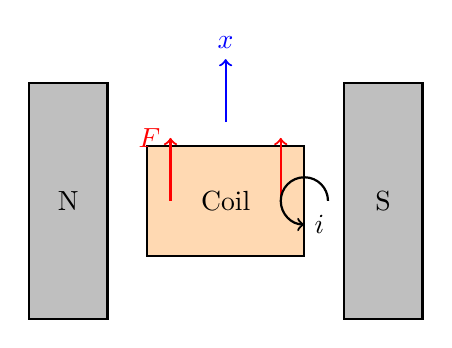
\begin{tikzpicture}
    % Magnet structure
    \draw[thick, fill=gray!50] (0,0) rectangle (1,3);
    \draw[thick, fill=gray!50] (4,0) rectangle (5,3);
    \node at (0.5,1.5) {N};
    \node at (4.5,1.5) {S};

    % Coil
    \draw[thick, fill=orange!30] (1.5,0.8) rectangle (3.5,2.2);
    \node at (2.5,1.5) {Coil};

    % Motion arrow
    \draw[->, thick, blue] (2.5,2.5) -- (2.5,3.3) node[above] {$x$};

    % Force arrows
    \draw[->, thick, red] (1.8,1.5) -- (1.8,2.3) node[left] {$F$};
    \draw[->, thick, red] (3.2,1.5) -- (3.2,2.3);

    % Current
    \draw[->, thick] (3.8,1.5) arc (0:270:0.3) node[right] {$i$};
\end{tikzpicture}
\caption{Voice coil actuator schematic.}
\label{fig:voice_coil}
\end{figure}

\textbf{Governing equations:}
\begin{align}
V &= Ri + L\frac{\dd i}{\dd t} + K_e\dot{x} \\
F &= K_f i = m\ddot{x} + b\dot{x}
\end{align}

Transfer function (voltage to position):
\begin{equation}
\frac{X(s)}{V(s)} = \frac{K_f}{s[(Ls + R)(ms + b) + K_f K_e]}
\end{equation}

% ============================================================================
\subsection{Solenoids}
\label{subsec:solenoids}
% ============================================================================

Solenoids provide on/off linear actuation. The force depends nonlinearly on position:

\begin{equation}
F = \frac{1}{2}i^2\frac{\dd L(x)}{\dd x}
\end{equation}

where $L(x)$ is the position-dependent inductance.

Linearized about operating point $(x_0, i_0)$:
\begin{equation}
\Delta F = K_i \Delta i + K_x \Delta x
\end{equation}

where $K_i$ and $K_x$ are partial derivatives of force with respect to current and position.

% ============================================================================
\subsection{Piezoelectric Actuators}
\label{subsec:piezo}
% ============================================================================

Piezoelectric actuators provide very small displacements (nm to $\mu$m) with high force and fast response.

\textbf{Constitutive equations:}
\begin{align}
x &= d_{33} V + s_{33} F/A \\
Q &= C V + d_{33} F
\end{align}

where:
\begin{itemize}
    \item $d_{33}$ = piezoelectric coefficient (m/V or C/N)
    \item $s_{33}$ = elastic compliance (m$^2$/N)
    \item $C$ = capacitance (F)
\end{itemize}

Transfer function (simplified, free displacement):
\begin{equation}
\frac{X(s)}{V(s)} = \frac{d_{33}\omega_n^2}{s^2 + 2\zeta\omega_n s + \omega_n^2}
\end{equation}

% ============================================================================
\subsection{Generators and Regeneration}
\label{subsec:generators}
% ============================================================================

When a motor is driven faster than its no-load speed, or when decelerating a load, it acts as a generator:

\begin{equation}
P_{\text{regen}} = e_b \cdot i_a = K_e\omega \cdot i_a
\end{equation}

This regenerated power can be:
\begin{itemize}
    \item Dissipated in braking resistors
    \item Returned to the power supply (regenerative braking)
    \item Stored in capacitors or batteries
\end{itemize}

% ============================================================================
\subsection{Motor Selection Example}
\label{subsec:motor_selection}
% ============================================================================

\begin{examplebox}[title=Example 1.9: Robot Joint Motor Selection]
A robot joint must:
\begin{itemize}
    \item Move a load with inertia $J_L = 0.05$ kg$\cdot$m$^2$
    \item Achieve maximum velocity $\omega_{\max} = 10$ rad/s
    \item Achieve maximum acceleration $\alpha_{\max} = 50$ rad/s$^2$
\end{itemize}

Select an appropriate motor and gear ratio.

\textbf{Solution:}

Required torque at load:
\begin{equation}
\tau_L = J_L \alpha_{\max} = 0.05 \times 50 = 2.5 \text{ N$\cdot$m}
\end{equation}

Consider a motor with:
\begin{itemize}
    \item Rated torque: $\tau_m = 0.3$ N$\cdot$m
    \item Rated speed: 3000 rpm = 314 rad/s
    \item Rotor inertia: $J_m = 5 \times 10^{-5}$ kg$\cdot$m$^2$
\end{itemize}

Required gear ratio (from torque):
\begin{equation}
n \geq \frac{\tau_L}{\tau_m} = \frac{2.5}{0.3} = 8.3
\end{equation}

Check speed (with $n = 10$):
\begin{equation}
\omega_m = n \cdot \omega_L = 10 \times 10 = 100 \text{ rad/s} < 314 \text{ rad/s} \quad \checkmark
\end{equation}

Reflected inertia check:
\begin{equation}
J_{\text{reflected}} = \frac{J_L}{n^2} = \frac{0.05}{100} = 5 \times 10^{-4} \text{ kg$\cdot$m$^2$}
\end{equation}

Total inertia at motor: $J_{\text{total}} = J_m + J_{\text{reflected}} = 5.5 \times 10^{-4}$ kg$\cdot$m$^2$

Motor acceleration:
\begin{equation}
\alpha_m = \frac{\tau_m}{J_{\text{total}}} = \frac{0.3}{5.5 \times 10^{-4}} = 545 \text{ rad/s}^2
\end{equation}

Load acceleration achieved:
\begin{equation}
\alpha_L = \frac{\alpha_m}{n} = \frac{545}{10} = 54.5 \text{ rad/s}^2 > 50 \text{ rad/s}^2 \quad \checkmark
\end{equation}

The motor with 10:1 gear ratio meets all requirements.
\end{examplebox}

% ============================================================================
\subsection{Exercises: Electromechanical Systems}
% ============================================================================

\begin{exercise}
A DC motor has $R_a = 1$ $\Omega$, $K_t = K_e = 0.05$ N$\cdot$m/A, $J = 2 \times 10^{-4}$ kg$\cdot$m$^2$, and $B = 10^{-4}$ N$\cdot$m$\cdot$s/rad. Neglect inductance.
\begin{enumerate}[label=(\alph*)]
    \item Derive the transfer function from voltage to velocity
    \item Find the steady-state speed for $V_a = 12$ V with no load
    \item Find the stall torque (torque at zero speed) for $V_a = 12$ V
\end{enumerate}
\end{exercise}

\begin{exercise}
For the motor in Exercise 1, a 5:1 gear reducer is added, and the load inertia is $J_L = 0.01$ kg$\cdot$m$^2$ with load damping $B_L = 0.01$ N$\cdot$m$\cdot$s/rad.
\begin{enumerate}[label=(\alph*)]
    \item Find the reflected load inertia and damping at the motor
    \item Derive the new transfer function from voltage to load velocity
    \item Compare the new time constant to the original
\end{enumerate}
\end{exercise}

\begin{exercise}
A voice coil actuator has $R = 5$ $\Omega$, $L = 1$ mH, $K_f = K_e = 10$ N/A, $m = 0.1$ kg, and $b = 2$ N$\cdot$s/m.
\begin{enumerate}[label=(\alph*)]
    \item Derive the transfer function from voltage to position
    \item Find all poles and determine if the system is stable
    \item Calculate the DC gain
\end{enumerate}
\end{exercise}

\begin{exercise}
A piezoelectric actuator has $d_{33} = 500$ pm/V, resonant frequency 30 kHz, and damping ratio 0.02.
\begin{enumerate}[label=(\alph*)]
    \item Write the transfer function
    \item Find the static displacement for 100V input
    \item Find the displacement amplitude at 20 kHz for 100V sinusoidal input
\end{enumerate}
\end{exercise}
